\section{Konzept und Umsetzung an der OTH-Regensburg}
\subsection{Vorstellung der OTH-Regensburg als Fallbeispiel}
Die Ostbayerische Technische Hochschule Regensburg (OTH-Regensburg) dient in
dieser Masterarbeit als praxisorientiertes Fallbeispiel für die Konzeption und 
Umsetzung eines innovativen Studiengangsfinders.

\subsubsection{Über die OTH-Regensburg}
Die OTH-Regensburg, gegründet im Jahr 1971, ist eine der größten Hochschulen
für angewandte Wissenschaften in Deutschland. Mit ihrem breiten Spektrum an 
praxisorientierten Studiengängen und ihrer engen Verbindung zur Industrie bietet
die OTH-Regensburg eine ideale Umgebung für die Entwicklung und Implementierung
eines innovativen Studiengangsfinders. \parencite{ueber-die-oth}

Die Hochschule zeichnet sich durch eine moderne Infrastruktur, hochqualifizierte 
Dozenten und eine enge Zusammenarbeit mit regionalen Unternehmen aus. Mit mehr
als 50 Bachelor- und Masterstudiengängen in den Bereichen
Ingenieurwissenschaften, Naturwissenschaften, Wirtschaft und
Sozialwissenschaften bietet die OTH-Regensburg eine breite Palette an 
Studienmöglichkeiten. \parencite{ueber-die-oth}

\subsubsection{Herausforderung und Zielsetzung}
Wie viele Bildungseinrichtungen steht auch die OTH-Regensburg vor der
Herausforderung, ihre Vielzahl an Studiengängen für Studieninteressierte
transparenter und zugänglicher zu machen. Der Studiengangsfinder, der im Rahmen
dieser Masterarbeit entwickelt wird, soll dazu beitragen, potenziellen
Studierenden eine klarere Orientierung über die verfügbaren Studienmöglichkeiten
zu bieten und ihre Entscheidungsfindung zu unterstützen.

Durch die Anwendung des Studiengangsfinders an der OTH-Regensburg wird nicht nur
ein innovatives Werkzeug für Studieninteressierte geschaffen, sondern auch die 
Effektivität und Transparenz der Studienorientierung an der Hochschule selbst 
verbessert. Die Integration und algorithmische Verarbeitung von Daten zu 
Studiengängen und Schwerpunkten ermöglicht eine präzisere Darstellung der 
Studienvielfalt und fördert gleichzeitig die strategische Ausrichtung der
Hochschule.

\subsection{Konzept für eine automatisch generierte Infografik}\label{sec:konzept}
Die Grundlage für das Konzept der automatisch generierten Infografik bildet die
methodische Vorarbeit, die in den vorhergehenden Kapiteln detailliert erläutert
wurde. Im Zuge der Methodik, wie in Kapitel \ref{sec:methodik} beschrieben,
wurden Studiengänge anhand verschiedener Kategorien bewertet und mithilfe des
MDS-Algorithmus in zweidimensionale Koordinaten transformiert. Das daraus
resultierende Zahlenmaterial bildet die Grundlage für die Visualisierung in der
Infografik. In den folgenden Unterkapiteln wird ein erstes Designkonzept für die
Software vorgestellt.

\subsubsection{Visualisierung der Studiengänge}

\begin{figure}[H]
    \centering
    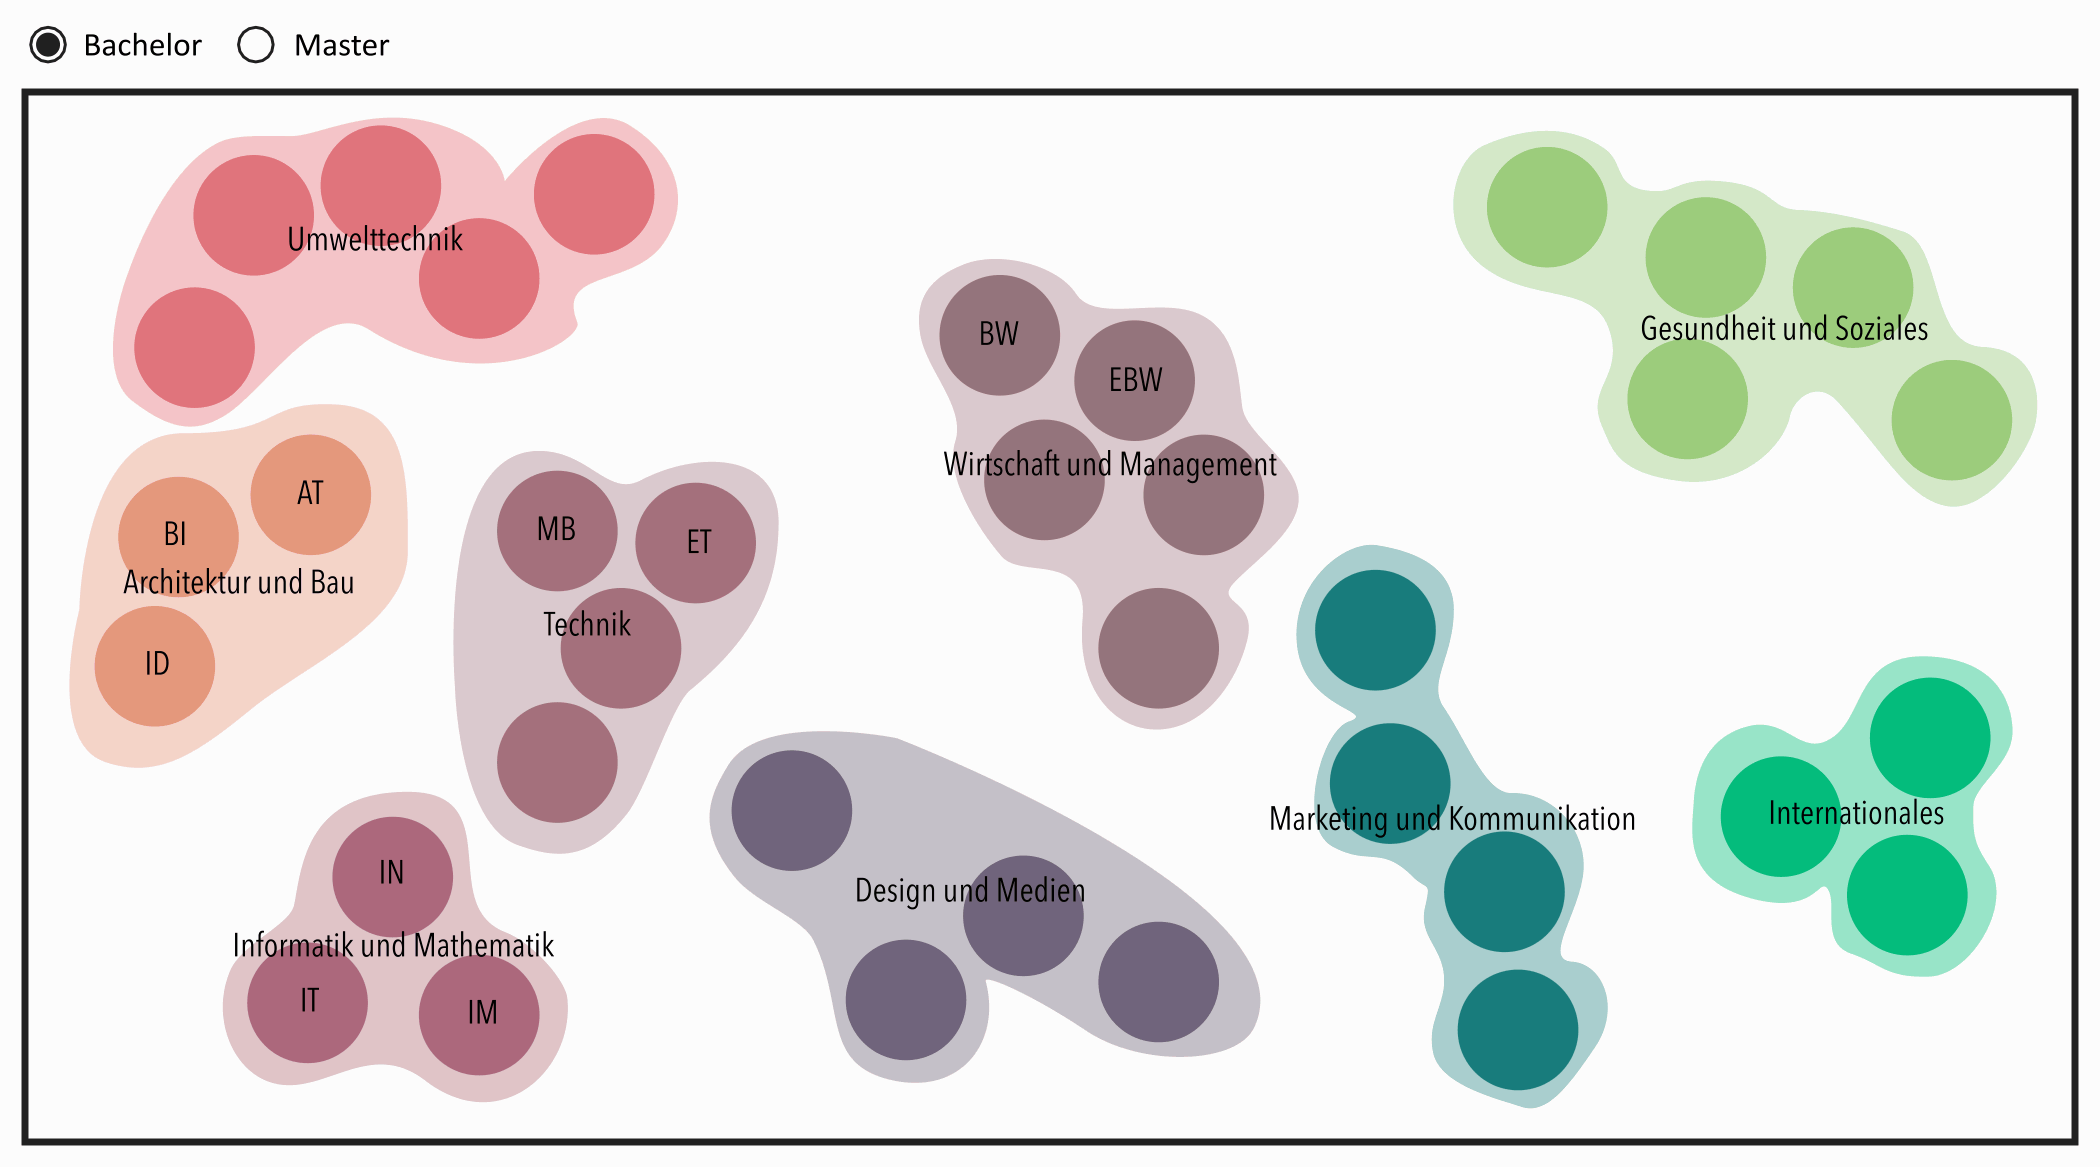
\includegraphics[width=\textwidth]{mockup_bubbles}
    \caption{Erstes Mockup einer möglichen Implementierung}
    \bildquelle{Eigene Darstellung}
    \label{fig:mockup-bubbles}
\end{figure}

Die automatisch generierte Infografik präsentiert die Vielfalt der Studiengänge
auf eine möglichst anschauliche Weise. Dabei werden inhaltlich ähnliche
Studiengänge in Form von sogenannten \glqq Bubbles\grqq{} in unmittelbarer Nähe 
zueinander positioniert (siehe \autoref{fig:mockup-bubbles}). Die Bubbles
enthalten jeweils die Kürzel der Studiengänge. Exemplarisch enthalten in
\autoref{fig:mockup-bubbles} nur einige wenige Bubbles ein Kürzel. Durch die
Verwendung von Pixi.js kann die resultierende Grafik dynamisch in allen Browsern,
die WebGL und Canvas unterstützen dargestellt werden.

\subsubsection{Berücksichtigung von Schwerpunkten}
Ein wesentlicher Aspekt des Infografik-Konzepts ist die Berücksichtigung von 
Schwerpunkten. Die Supergruppen, die in der Datenverarbeitung definiert wurden, 
werden hier als leichter Schleier um die darin beinhalteten Studiengänge 
präsentiert (siehe \autoref{fig:mockup-bubbles}). Außerdem werden alle
Supergruppen mit einer zentrierten Beschriftung versehen. Dies ermöglicht es den
Nutzern, gezielt nach Studiengängen innerhalb bestimmter Kategorien zu suchen
und ihre Präferenzen entsprechend auszurichten.

\subsubsection{Interaktivität}
Die Infografik wird durch interaktive Elemente angereichert, um den Nutzern eine
individuelle Erkundung der Daten zu ermöglichen. Beispielsweise können durch
Mausklicks zusätzliche Informationen zu einem Studiengang abgerufen werden.

\begin{figure}[H]
    \centering
    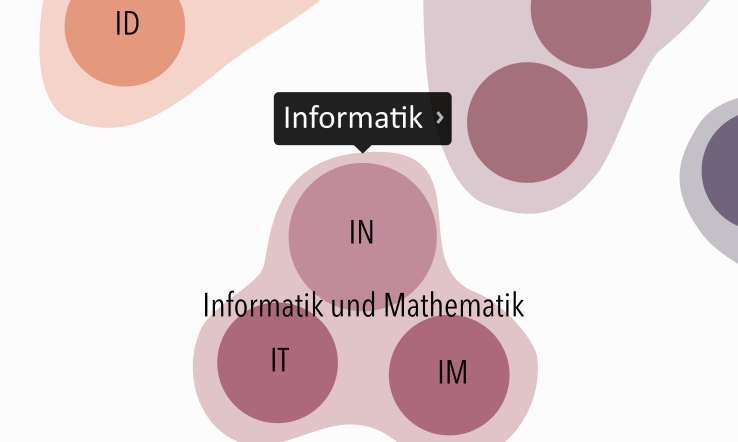
\includegraphics[width=0.5\textwidth]{mockup_bubbles_hover}
    \caption{Mockup: Tooltip über Bubble}
    \bildquelle{Eigene Darstellung}
    \label{fig:mockup-bubbles-hover}
\end{figure}

Sobald ein Benutzer auf einem Desktop-Gerät (z.B. Laptop) mit der Maus über eine
Bubble fährt, erscheint ein Tooltip mit dem vollständigen Namen des Studiengangs
(siehe \autoref{fig:mockup-bubbles-hover}). Ein Tooltip ist ein grafisches
Element, das kurze Textinformationen liefert. Aufgrund der fehlenden Maus auf
mobilen Endgeräten, erscheint der Tooltip darauf erst beim Klick auf eine
Bubble. 

Möchte der Studieninteressierte mehr über den Studiengang erfahren, bietet das
Konzept zusätzlich die Möglichkeit, ein Popup mit Details zu öffnen (siehe
\autoref{fig:mockup-bubbles-popup}). Bei Desktop-Geräten genügt ein einfacher
Klick auf die Sprechblase oder den sich öffnenden Tooltip, bei mobilen
Endgeräten ist ein zweiter Klick auf die jeweiligen Elemente erforderlich.

\begin{figure}[H]
    \centering
    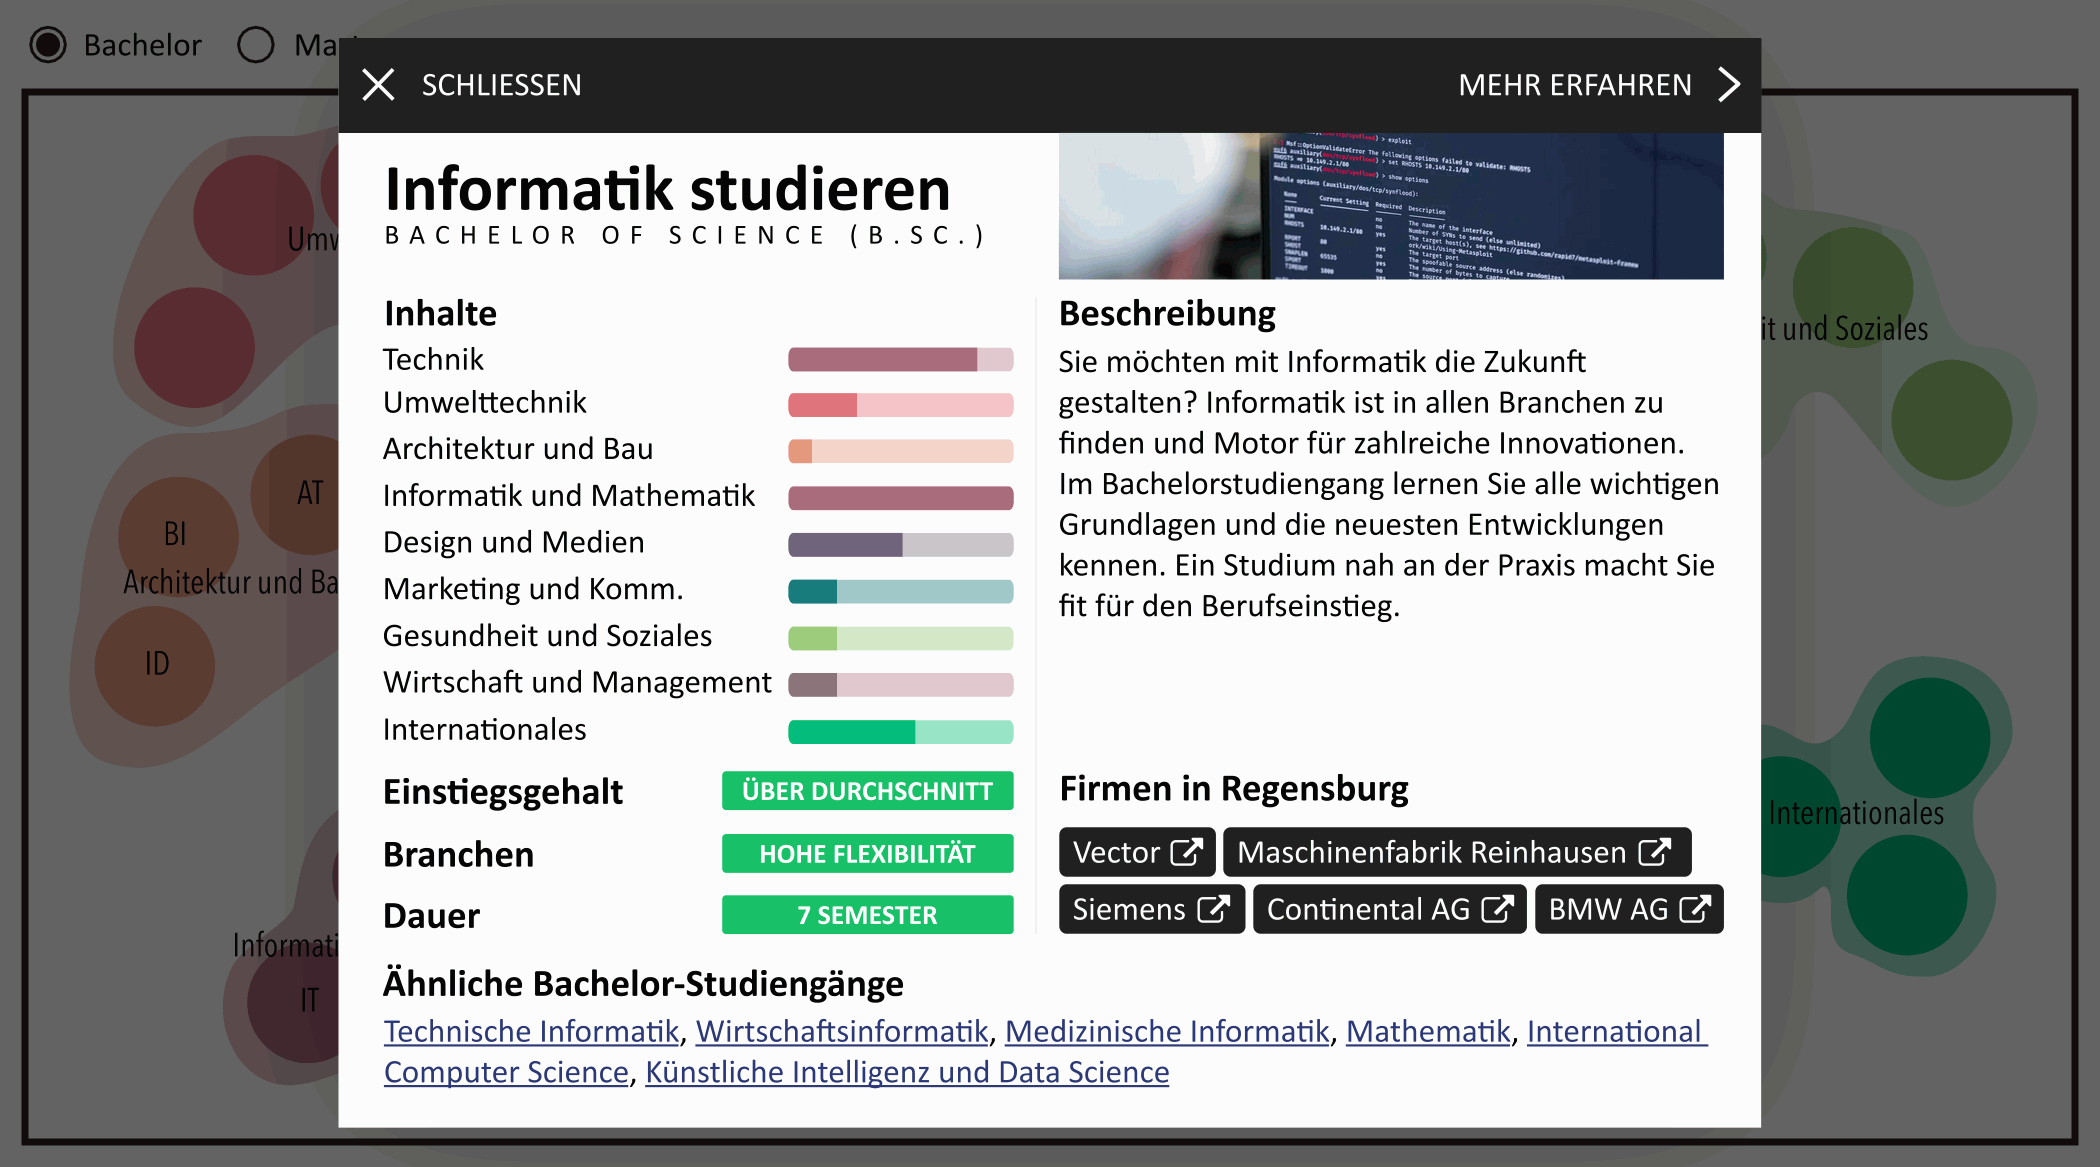
\includegraphics[width=\textwidth]{mockup_bubbles_popup}
    \caption{Mockup: Popup mit Details eines Studiengangs}
    \bildquelle{Eigene Darstellung}
    \label{fig:mockup-bubbles-popup}
\end{figure}

Im Folgenden wird das Konzept des Popup-Dialogs beschrieben, das in
\autoref{fig:mockup-bubbles-popup} visualisiert ist.

Innerhalb des Popups findet der Nutzer eine prägnante Kurzbeschreibung des 
Studiengangs. Die Inhalte werden durch Fortschrittsbalken visualisiert, die den
Anteil der verschiedenen Kategorien darstellen. So kann beispielsweise die
Kategorie \glqq Informatik\grqq{} zu 90\% ausgefüllt sein, um den Schwerpunkt
des Studiengangs zu verdeutlichen.

Zusätzlich liefert das Popup Informationen über Einstiegsgehälter, relevante
Branchen, Studiendauer und ähnliche Studiengänge. Letztere werden nicht statisch 
dargestellt, sondern vom Algorithmus dynamisch berechnet, um stets aktuelle und
präzise Informationen zu liefern.

Außerdem enthält der Dialog eine Liste von Unternehmen in Regensburg, die
gezielt nach Absolventen dieses Studiengangs suchen. Dieser Aspekt gibt dem
Nutzer einen Einblick in potentielle Arbeitgeber und eröffnet berufliche
Perspektiven direkt in der Region.

Durch die Integration dieses Fensters wird die Benutzerfreundlichkeit erheblich 
verbessert, da der Nutzer einen tieferen Einblick in die einzelnen Studiengänge
erhält, ohne die Seite wechseln zu müssen.

\subsection{User-centered Design Research: Mockup eines Prototypen}

\subsubsection{Allgemeines}
Bei der Entwicklung eines nutzerzentrierten Designs steht die direkte Einbindung
der Zielgruppe im Mittelpunkt. Dieser Ansatz, der als User-Centered Design (UCD) 
bezeichnet wird, stellt die Integration der Bedürfnisse, Erwartungen und
Anforderungen der Benutzer in den Entwicklungsprozess in den Mittelpunkt. Ziel
ist es, Produkte und Anwendungen zu gestalten, die nicht nur funktional und
ästhetisch ansprechend sind, sondern auch die bestmögliche
Benutzerfreundlichkeit bieten.

\subsubsection{Methode und Teilnehmende}
Im Rahmen des UCD-Prozesses wurde das zuvor in Kapitel \ref{sec:konzept}
vorgestellte Mockup-Konzept für den Studiengangsfinder entwickelt, das als
Prototyp diente. Um sicherzustellen, dass das entworfene Konzept den
Bedürfnissen der potenziellen Nutzer entspricht, wurde eine gezielte 
User-Centered-Design-Studie durchgeführt. Zu diesem Zweck wurden sechs
Absolventen verschiedener Fachrichtungen eingeladen, den Prototyp zu evaluieren.

\subsubsection{Ablauf des Tests}
Die Studienteilnehmer wurden ermutigt, ihre persönlichen Perspektiven,
Erfahrungen und Vorschläge einzubringen. Offene Fragen zu Designelementen,
Verständlichkeit von Informationen und allgemeinen Nutzererfahrungen sollte
Einblicke in mögliche Stärken und Schwächen des Prototyps geben. Ziel war es, 
frühzeitig wertvolles Feedback zu erhalten, um Optimierungen und Anpassungen
vornehmen zu können, bevor die Implementierung in die nächste Phase ging.

\subsubsection{Ergebnisse}

\subsection{Beschreibung der Positionsberechnung der Infografik}

\subsection{Technische Details zur Umsetzung}

\subsection{Anwendung des entwickelten Systems auf die Studiengänge der OTH-Regensburg}